\section{Introduction}

Month-to-month air temperature in Central Europe is dominated by a strong, nearly deterministic annual cycle, on top of which irregular anomalies of roughly two degrees Celsius obscure any slow change in the mean. For planners in municipal heat management, energy supply, and agriculture, this creates a concrete forecasting question: at horizons of up to three years, does a statistical model add anything to the heuristic of reusing the value from the same month one year earlier? We study this question for monthly mean air temperature at 2 metres in Frankfurt am Main, using NASA POWER data \citep{NASA_POWER} for the grid cell centred at 50.11$^\circ$N, 8.68$^\circ$E from January 1981 to December 2025.

This paper addresses two descriptive and predictive questions. First, how has the monthly mean temperature in Frankfurt changed since 1981, in its overall level, across seasons, and in the amplitude and phase of the seasonal cycle? Second, how well do seasonal forecasting models predict the 36 months of a fixed hold-out relative to a seasonal naive baseline? We make no causal claim. All trend estimates are associations with calendar time, and the forecasting comparison evaluates predictive accuracy only.

Our design fixes the forecast setup before any model is fitted. Models are estimated on January 1981 to December 2022 (504 months) and evaluated on the final 36 months, January 2023 to December 2025. We compare two baselines (seasonal naive and naive) with four candidates: additive Holt-Winters exponential smoothing without trend, ETS(A,N,A), and with damped trend, ETS(A,Ad,A); a seasonal ARIMA model with orders chosen on the training window; and a regression on a linear trend and annual harmonics. Accuracy is measured by RMSE, MAE, and MASE, and differences against the seasonal naive baseline are tested with the Diebold-Mariano test. We report every declared model, including those that lose to the baseline.

Our findings can be summarised as follows. Annual mean temperature in Frankfurt rose by about 0.50 degrees Celsius per decade over 1981--2022, and the warming appears in all four seasons, with the largest estimates in winter and summer. We find no evidence that the amplitude or phase of the seasonal cycle changed. On the hold-out, all four candidate models reduce the root mean squared error of the seasonal naive baseline by roughly 30 percent, and the differences are statistically significant at the 5 percent level, although the short hold-out limits the power of this comparison. The naive last-value forecast is far worse than the seasonal naive baseline. The four candidates are statistically indistinguishable from one another.

The paper makes a modest contribution of three kinds. First, it provides a transparent and reproducible local trend estimate with explicit uncertainty for a reanalysis grid cell in the Rhine-Main region. Second, it quantifies the forecast gain of simple statistical models over a heuristic that practitioners commonly use, with a setup frozen before estimation. Third, it documents the calibration of the prediction intervals on the hold-out, which shows that model-based intervals are substantially narrower than those of the baseline while maintaining near-nominal coverage.

The remainder of this study is structured as follows: Section~2 describes the data, Section~3 the empirical strategy, Section~4 the results, and Section~5 discusses implications and limitations.

\section{Data}

\subsection{NASA POWER and the Frankfurt grid cell}

We use the monthly 2 metre air temperature (T2M) from the NASA Prediction of Worldwide Energy Resources (POWER) project \citep{NASA_POWER}. POWER derives its meteorological parameters from the MERRA-2 reanalysis, which assimilates observations into a global atmospheric model on a regular grid. The series is therefore a grid-cell reanalysis value for the cell containing 50.11$^\circ$N, 8.68$^\circ$E, not a station record. Local effects such as the urban heat island of Frankfurt, and any differences between the grid-cell elevation and the elevation of a measuring site, are only partly represented. Absolute levels and trends should consequently be read as properties of the reanalysis cell, and not as those of an individual weather station.

\subsection{Sample and variables}

The sample contains 540 monthly observations from January 1981 to December 2025.
% src: summary_statistics.json#n_observations
% src: summary_statistics.json#time_coverage.n_periods
The data end in December 2025 because the POWER monthly load covers whole calendar years. No observation is missing, no fill values occur, and all 45 years are complete.
% src: summary_statistics.json#completeness.n_years
% src: summary_statistics.json#completeness.n_incomplete_years
We split the sample at a fixed origin: the 504 months from 1981-01 to 2022-12 form the training window, and the 36 months from 2023-01 to 2025-12 form the hold-out.
% src: summary_statistics.json#split.n_train
% src: summary_statistics.json#split.n_holdout
The mean monthly temperature is 9.94 degrees Celsius with a standard deviation of 7.54, reflecting the annual cycle.
% src: summary_statistics.json#outcome.T2M.mean
% src: summary_statistics.json#outcome.T2M.sd
The training mean is 9.83 degrees, whereas the hold-out mean is 11.46 degrees, which already indicates that the hold-out period is warmer than the average of the training window.
% src: summary_statistics.json#outcome_train.T2M.mean
% src: summary_statistics.json#outcome_holdout.T2M.mean
Anomalies relative to the 1981--2010 monthly climatology have a standard deviation of 1.90 degrees over the full sample and a mean of 0.44 degrees.
% src: summary_statistics.json#anomaly_full.sd
% src: summary_statistics.json#anomaly_full.mean
Decade means of the annual temperature rise from 9.09 degrees in 1981--1990 to 11.19 degrees in 2021--2025.
% src: summary_statistics.json#decade_means.1981_1990
% src: summary_statistics.json#decade_means.2021_2025
Figure~\ref{fig:monthly} shows the monthly series and Figure~\ref{fig:annual} the annual means.

\begin{figure}[t]
\centering
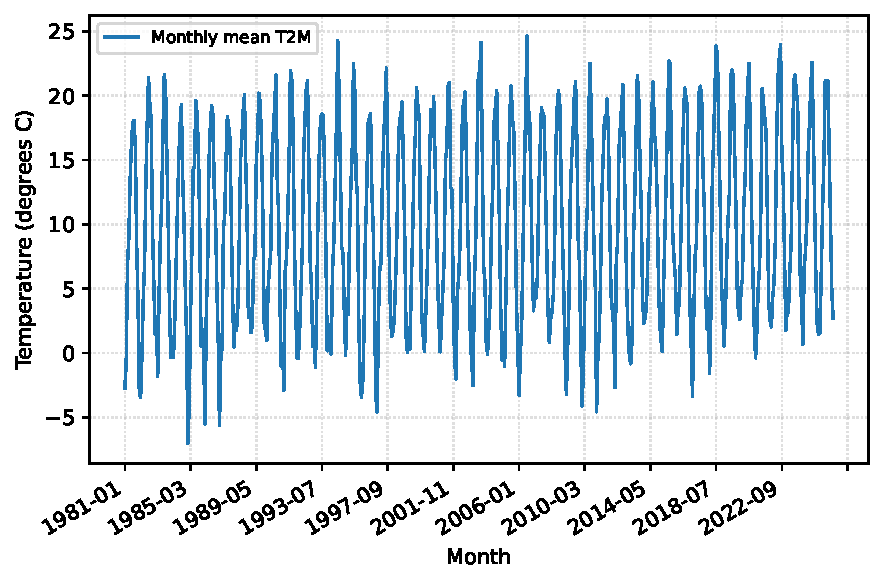
\includegraphics[width=0.95\textwidth]{fig_monthly_t2m.pdf}
\caption{Monthly mean 2 m air temperature, Frankfurt am Main grid cell (NASA POWER), 1981--2025.}
\label{fig:monthly}
\end{figure}

\begin{figure}[t]
\centering
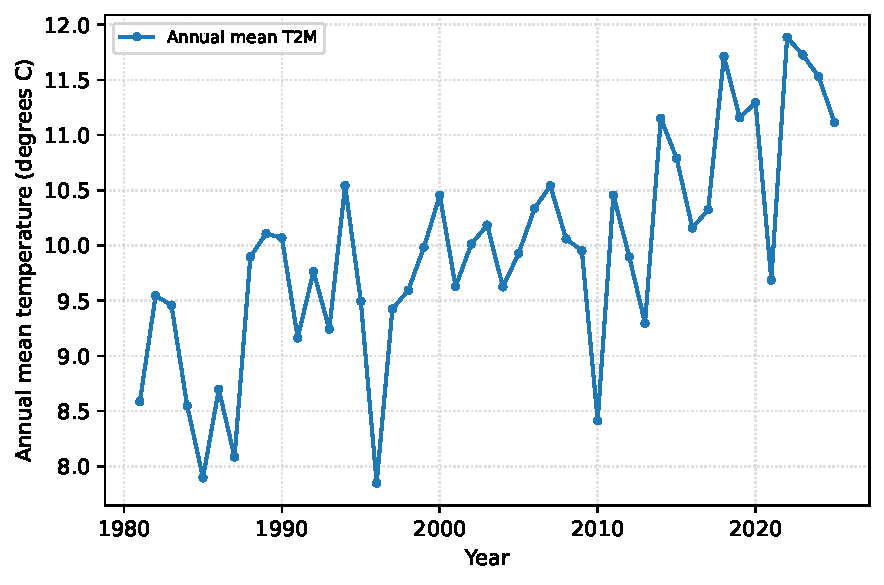
\includegraphics[width=0.95\textwidth]{fig_annual_means.pdf}
\caption{Annual mean 2 m air temperature, Frankfurt am Main grid cell (NASA POWER), 1981--2025.}
\label{fig:annual}
\end{figure}

\section{Empirical Strategy}

\subsection{Trend description}

We describe the long-run change in three ways, all on the training years 1981--2022 and, for comparison, on the full sample. First, we regress annual mean temperature on calendar year by OLS with Newey-West (HAC) standard errors. Second, we repeat this on the deseasonalised monthly series, which removes calendar-month means. Third, we estimate season-specific slopes for December--February, March--May, June--August, and September--November. Because the annual regression is estimated on only 42 observations, we complement it with the nonparametric Mann-Kendall test \citep{mann1945nonparametric} and Sen's slope \citep{sen1968estimates}, including an autocorrelation-corrected variant. We also test whether the amplitude and phase of the annual harmonic drift linearly over time, using a joint HAC Wald test. These estimates describe associations with calendar time and do not identify causes of warming.

\subsection{Stationarity diagnostics}

We apply the Augmented Dickey-Fuller test \citep{dickey1979distribution} and the KPSS test \citep{kwiatkowski1992testing} to the seasonally adjusted training series. Reading both tests together is informative: the ADF test has a unit root as null hypothesis, whereas KPSS has stationarity as null. All diagnostics are computed on data up to December 2022 and therefore do not use the hold-out.

\subsection{Forecasting models and evaluation}

The forecast setup was fixed before estimation and frozen together with the hold-out. The two baselines are the seasonal naive forecast (the value twelve months earlier) and the naive forecast (the last observed value) \citep{hyndman2021forecasting}. The four candidates are ETS(A,N,A) and ETS(A,Ad,A), i.e., additive Holt-Winters exponential smoothing without and with a damped trend; a seasonal ARIMA model \citep{box2008time} whose orders are chosen on the training window by AICc in a stepwise search in the spirit of \citet{hyndman2008automatic}; and an OLS regression on a linear trend and annual harmonics, with the number of harmonics chosen by AICc. Model choice uses the training window only. Every model is fitted at the origin December 2022 and forecasts the 36 months of the hold-out in a single pass, so that all hold-out errors are genuine out-of-sample errors \citep{tashman2000out}. Prediction intervals are at the 95 percent level, and we report the share of hold-out values that fall inside them.

We measure accuracy by RMSE and MAE in degrees Celsius and by the mean absolute scaled error (MASE), which scales the MAE by the in-sample MAE of the seasonal naive method on the training window \citep{hyndman2006another}. This scale is 2.04 degrees.
% src: estimation_results.json#series.mase_scale_seasonal_naive_mae_train
To test whether a candidate forecasts better than the seasonal naive baseline, we use the Diebold-Mariano test \citep{diebold1995comparing} with the small-sample correction of \citet{harvey1997testing}, applied to squared and absolute error differences over the 36 hold-out months. A rolling-origin exercise inside the training window (twenty annual origins from December 2000 to December 2019, each with a 36-month horizon) supplements the single hold-out; because these origins overlap, we use it to assess horizon and season structure and not to select models. Finally, each model is refitted on all 540 months to produce forecasts for January 2026 to December 2028, which are not evaluated.

We stated three expectations before seeing the results. The first (H1) was a positive annual trend of between 0.3 and 0.5 degrees per decade. The second (H2) was that the candidate models improve on the seasonal naive baseline. The third (H3) was that the trend-based models and the exponential smoothing and ARIMA models do not differ significantly on a three-year hold-out. We evaluate them in Section~4 without revision.

\section{Results}

\subsection{Trend, seasonality, and stationarity}

Annual mean temperature in Frankfurt increased by 0.50 degrees Celsius per decade over 1981--2022 (HAC standard error 0.08, 95 percent confidence interval 0.34 to 0.67).
% src: estimation_results.json#trend.annual_training_1981_2022.slope_per_decade
% src: estimation_results.json#trend.annual_training_1981_2022.se_per_decade
% src: estimation_results.json#trend.annual_training_1981_2022.ci_lower_per_decade
% src: estimation_results.json#trend.annual_training_1981_2022.ci_upper_per_decade
The point estimate lies marginally above the range of 0.3 to 0.5 degrees that we stated in advance for H1, so the hypothesis is supported in sign but not fully in magnitude; the lower end of the confidence interval nevertheless lies inside the stated range. The slope from the deseasonalised monthly series is practically identical at 0.50 degrees per decade, and extending the sample to 2025 raises the annual estimate to 0.54 degrees per decade.
% src: estimation_results.json#trend.deseasonalised_monthly_training_1981_2022.slope_per_decade
% src: estimation_results.json#trend.annual_full_1981_2025.slope_per_decade
The Mann-Kendall test confirms a monotone upward trend in annual means (statistic 4.48, $p<0.001$) with a Sen slope of 0.50 degrees per decade; the variance adjustment for autocorrelation leaves the statistic unchanged, since the estimated variance inflation factor equals one (Table~\ref{tab:diag}).
% src: estimation_results.json#diagnostics.mann_kendall_annual.statistic
% src: estimation_results.json#diagnostics.mann_kendall_annual.sen_slope_per_decade
% src: estimation_results.json#diagnostics.mann_kendall_annual.variance_inflation

Warming appears in every season (Table~\ref{tab:seasons}). Over the training years, the slope is 0.62 degrees per decade in winter and 0.61 in summer, compared with 0.38 in spring and 0.39 in autumn.
% src: estimation_results.json#trend.seasonal_training_1981_2022.DJF.slope_per_decade
% src: estimation_results.json#trend.seasonal_training_1981_2022.JJA.slope_per_decade
% src: estimation_results.json#trend.seasonal_training_1981_2022.MAM.slope_per_decade
% src: estimation_results.json#trend.seasonal_training_1981_2022.SON.slope_per_decade
The confidence intervals of the four seasons overlap substantially, so the data do not support a claim that the seasons warm at different rates. The seasonal cycle itself is stable: the fitted amplitude of the annual harmonic changes by $-0.15$ degrees and the phase by $-1.6$ degrees between the start and end of the training window, and the joint Wald test of both drift terms does not reject constancy ($p=0.76$).
% src: estimation_results.json#trend.seasonal_cycle_drift_training.amplitude_change_degC
% src: estimation_results.json#trend.seasonal_cycle_drift_training.phase_shift_deg
% src: estimation_results.json#trend.seasonal_cycle_drift_training.joint_wald_p

\input{tables/seasons.tex}

The stationarity tests, computed on the seasonally adjusted training series, give a mixed but interpretable picture. The ADF test rejects a unit root (statistic $-6.87$), whereas the KPSS test rejects level stationarity (statistic 1.99, $p$-value bounded at 0.01).
% src: estimation_results.json#diagnostics.adf_seasonally_adjusted.statistic
% src: estimation_results.json#diagnostics.kpss_level.statistic
% src: estimation_results.json#diagnostics.kpss_level.p_value
Rejection by both tests points to trend-stationary behaviour, i.e., fluctuations around a slowly rising mean and not a random walk, which is consistent with the trend estimates above.

\input{tables/diag.tex}

\subsection{Hold-out forecast accuracy}

Table~\ref{tab:oos} reports the out-of-sample accuracy of all six models on the 36 hold-out months. The seasonal naive baseline attains an RMSE of 1.92 degrees Celsius, an MAE of 1.64 degrees, and a MASE of 0.80.
% src: estimation_results.json#out_of_sample.seasonal_naive_test.rmse
% src: estimation_results.json#out_of_sample.seasonal_naive_test.mae
% src: estimation_results.json#out_of_sample.seasonal_naive_test.mase
The naive last-value forecast performs far worse, with an RMSE of 12.06 degrees and a MASE of 4.79, because it ignores the annual cycle entirely; it loses to the seasonal naive baseline by a wide margin, and its Diebold-Mariano statistics are strongly negative.
% src: estimation_results.json#out_of_sample.naive_test.rmse
% src: estimation_results.json#out_of_sample.naive_test.mase
% src: estimation_results.json#dm_tests.naive.squared_h12.statistic
All four candidates beat the seasonal naive baseline. ETS(A,Ad,A) has the lowest RMSE (1.30 degrees), followed closely by ETS(A,N,A) (1.30), the harmonic trend regression (1.36), and SARIMA (1.37). Their MASE values lie between 0.48 and 0.50.
% src: estimation_results.json#out_of_sample.ets_aada_test.rmse
% src: estimation_results.json#out_of_sample.ets_ana_test.rmse
% src: estimation_results.json#out_of_sample.harmonic_trend_test.rmse
% src: estimation_results.json#out_of_sample.sarima_test.rmse
% src: estimation_results.json#out_of_sample.ets_ana_test.mase
% src: estimation_results.json#out_of_sample.harmonic_trend_test.mase
The RMSE ratio relative to seasonal naive is 0.68 for both exponential smoothing variants and 0.71 for SARIMA and the harmonic regression.
% src: estimation_results.json#h2_result.models.ets_ana.holdout_rmse_ratio_vs_seasonal_naive
% src: estimation_results.json#h2_result.models.sarima.holdout_rmse_ratio_vs_seasonal_naive
% src: estimation_results.json#h2_result.models.harmonic_trend.holdout_rmse_ratio_vs_seasonal_naive
We therefore find support for H2 on the hold-out.

\input{tables/oos.tex}

Table~\ref{tab:dm} shows that the improvements are statistically significant but not overwhelming. With the Harvey-Leybourne-Newbold correction and squared-error loss, the Diebold-Mariano statistic against seasonal naive is 2.75 for ETS(A,N,A) ($p=0.009$), 2.75 for ETS(A,Ad,A) ($p=0.009$), 2.47 for the harmonic regression ($p=0.019$), and 2.17 for SARIMA ($p=0.037$).
% src: estimation_results.json#dm_tests.ets_ana.squared_h12.statistic
% src: estimation_results.json#dm_tests.ets_ana.squared_h12.p_value
% src: estimation_results.json#dm_tests.ets_aada.squared_h12.p_value
% src: estimation_results.json#dm_tests.harmonic_trend.squared_h12.statistic
% src: estimation_results.json#dm_tests.harmonic_trend.squared_h12.p_value
% src: estimation_results.json#dm_tests.sarima.squared_h12.statistic
% src: estimation_results.json#dm_tests.sarima.squared_h12.p_value
Absolute-error loss gives the same ranking and conclusions. With only 36 monthly errors that are serially dependent, the test has limited power and the p-values should be read as indicative. Pairwise tests among the candidates reveal no significant difference: the smallest $p$-value is 0.18 (ETS(A,Ad,A) against the harmonic regression), and none of the three pairs is significant at the 5 percent level, which supports H3.
% src: estimation_results.json#h3_result.pairwise_dm.ets_aada_vs_harmonic_trend.p_value
% src: estimation_results.json#h3_result.n_pairs_significant_5pct

\input{tables/dm.tex}

\subsection{Prediction intervals}

The 95 percent intervals of the seasonal naive baseline cover all 36 hold-out values (coverage 100 percent), but they are wide, with a mean width of 14.2 degrees.
% src: estimation_results.json#out_of_sample.seasonal_naive_test.coverage
% src: estimation_results.json#out_of_sample.seasonal_naive_test.mean_interval_width
The candidate models cover 35 of the 36 values (97.2 percent) with intervals that are about half as wide (mean width 7.2 to 7.3 degrees).
% src: estimation_results.json#out_of_sample.ets_ana_test.coverage
% src: estimation_results.json#out_of_sample.ets_ana_test.mean_interval_width
% src: estimation_results.json#out_of_sample.sarima_test.mean_interval_width
Coverage is thus close to nominal for the candidates and conservative for the baseline, whose interval inflates the uncertainty of a single seasonal difference. With 36 observations, a coverage rate of 97 percent cannot be distinguished from 95 percent.

\subsection{Horizon and season structure}

The error of the seasonal naive baseline is flat across horizons: RMSE is 1.92 degrees in months 1 to 12, 1.94 in months 13 to 24, and 1.89 in months 25 to 36.
% src: estimation_results.json#out_of_sample.seasonal_naive_test.by_horizon_block.h01_12.rmse
% src: estimation_results.json#out_of_sample.seasonal_naive_test.by_horizon_block.h13_24.rmse
% src: estimation_results.json#out_of_sample.seasonal_naive_test.by_horizon_block.h25_36.rmse
This is expected because its forecast does not depend on the horizon beyond the interval width. The relative advantage of the candidates is largest in the final year of the hold-out, where their RMSE is about 43 to 46 percent of the baseline's.
% src: estimation_results.json#h2_result.models.ets_ana.holdout_rmse_ratio_h25_36
% src: estimation_results.json#h2_result.models.harmonic_trend.holdout_rmse_ratio_h25_36
This pattern coincides with the warm years 2023 to 2025 and is consistent with the level shift that the baseline, anchored on a single past year, cannot track; with only three hold-out years, however, we cannot separate this from chance.

The rolling-origin exercise in the training window gives a less favourable picture for the seasonal naive baseline and a more modest one for the candidates. Across twenty overlapping origins, the baseline's MASE is 1.02, whereas the candidate models reach MASE values between 0.71 and 0.73.
% src: estimation_results.json#rolling_origin.seasonal_naive.mase_overall
% src: estimation_results.json#h2_result.models.harmonic_trend.rolling_mase
% src: estimation_results.json#h2_result.models.ets_aada.rolling_mase
In the rolling exercise, the RMSE ratio at horizons 25 to 36 is between 0.71 and 0.73.
% src: estimation_results.json#h2_result.models.harmonic_trend.rolling_relative_rmse_h25_36
% src: estimation_results.json#h2_result.models.ets_aada.rolling_relative_rmse_h25_36
Hence the advantage of the candidates over seasonal naive is reproduced outside the final hold-out, and it is smaller than on the 2023--2025 window.

\subsection{Forecasts beyond the data}

Refitted on all 540 months, the harmonic regression estimates a linear trend of 0.054 degrees per year.
% src: estimation_results.json#models.harmonic_trend_full.parameters.trend_years.estimate
The forecasts for January 2026 to December 2028 are stored for all six models in the results file with 95 percent intervals. Because these forecasts lie beyond the data, they cannot be evaluated here, and we do not interpret them as predictions of any particular year.

\section{Discussion and Conclusion}

Monthly mean air temperature in the Frankfurt reanalysis grid cell rose by about 0.5 degrees Celsius per decade between 1981 and 2022, with all four seasons contributing and no detectable change in the amplitude or phase of the annual cycle. On a hold-out of 36 months, simple statistical models that combine the seasonal pattern with a slowly moving level or a linear trend reduce the RMSE of the seasonal naive baseline by around 30 percent, and these gains are significant at the 5 percent level but not decisive given the short hold-out. The choice among exponential smoothing, SARIMA, and a harmonic regression does not matter for accuracy at this horizon. The naive last-value forecast is unsuitable for monthly temperature.

For practitioners, the results suggest that reusing last year's value is a defensible but costly heuristic: a trend-aware seasonal model delivers a lower error and intervals about half as wide at comparable coverage. Because the three-year hold-out coincides with a warm period, the size of the gain is likely larger than in an average three-year window; the rolling-origin results, with an RMSE ratio near 0.72 at the longest horizons, provide a more conservative reference. For scholars, the study documents that the trend of roughly 0.5 degrees per decade is large enough relative to interannual variability to be exploited at a three-year horizon, but only modestly so.

Our analysis is subject to several scope conditions. The data are a MERRA-2 reanalysis grid cell, not a station record, so trends and levels may differ from those measured at a weather station; a comparison with station observations from the German Weather Service (DWD) is a natural extension but is not part of this study, and no DWD data are used here. The hold-out contains only 36 serially dependent months, which limits the power of the Diebold-Mariano comparisons and the precision of the coverage estimates. Finally, the trend estimates are associations with calendar time and the analysis makes no claim about the causes of warming.

Future research could ask whether the gain from trend-aware models over seasonal naive persists when the models are evaluated against DWD station observations, and whether the horizon-specific skill pattern holds across several grid cells in Germany.

\bibliographystyle{apalike}
\bibliography{literature}
